% !TEX program = xelatex
%-----------------------------------
% Beamer template style: Madrid + rose
% xelatex
%-----------------------------------

\documentclass[UTF8,aspectratio=169,11pt]{ctexbeamer}

\mode<presentation>{
  \usetheme{Madrid}
  \usecolortheme{rose}
  \setbeamertemplate{navigation symbols}{}
}

\usepackage{fontspec}
\usepackage{graphicx}
\usepackage{booktabs}
\usepackage{tabularx}
\usepackage{array}
\usepackage{tikz}
\usetikzlibrary{arrows.meta,positioning}
\usepackage{listings}
\usepackage[bookmarks=true]{hyperref}

\graphicspath{{fig/}}

\IfFontExistsTF{Microsoft YaHei UI}{
  \setCJKmainfont{Microsoft YaHei UI}
  \setCJKsansfont{Microsoft YaHei UI}
}{}
\IfFontExistsTF{Consolas}{\setmonofont{Consolas}}{}

\lstset{
  basicstyle=\ttfamily\scriptsize,
  keywordstyle=\bfseries,
  frame=single,
  breaklines=true,
  showstringspaces=false,
  columns=fullflexible,
  tabsize=2
}

\newcolumntype{Y}{>{\raggedright\arraybackslash}X}
\newcommand{\takeaway}[1]{\begin{block}{本页结论}#1\end{block}}
\newcommand{\smallpoint}[2]{\textbf{#1}\par{\small #2}\par\vspace{0.35em}}

\title[协程技术调研]{协程技术调研}
\subtitle{从并发演进到底层机制、语言选型与实验验证}
\author[柯云超]{柯云超}
\institute[并行程序设计]{计算机学院 \\ \medskip \textit{并行程序设计课程展示}}
\date{2026 年 6 月}

\begin{document}

\begin{frame}
  \titlepage
\end{frame}

\begin{frame}
  \frametitle{Overview}
  \tableofcontents
\end{frame}

\section{引言：协程解决的是等待方式}

\begin{frame}{核心判断：让等待更便宜}
  \begin{columns}[T,totalwidth=\linewidth]
    \begin{column}{0.56\linewidth}
      {\LARGE\bfseries 协程降低的是“等待”的代价，\\不是“计算”的代价。\par}
      \vspace{0.35cm}
      对网络服务而言，很多请求大部分时间在等数据库、磁盘、网络或 RPC。协程把等待中的任务从昂贵的内核线程上挪开，同时保留接近同步代码的控制流。
    \end{column}
    \begin{column}{0.38\linewidth}
      \begin{block}{本次汇报主线}
        \begin{enumerate}
          \item 为什么从线程走向协程？
          \item 有栈/无栈到底保存什么？
          \item 主流语言路线为何不同？
          \item 实验能证明哪些边界？
        \end{enumerate}
      \end{block}
    \end{column}
  \end{columns}
\end{frame}

\begin{frame}{并发模型演进：等待任务越来越多}
  \centering
  \begin{tikzpicture}[
    node distance=0.85cm,
    box/.style={draw, rounded corners=2pt, minimum width=2.25cm, minimum height=1.05cm, align=center},
    arr/.style={-{Stealth[length=2.4mm]}, thick}
  ]
    \node[box] (proc) {\bfseries 多进程\\{\scriptsize 隔离强，通信贵}};
    \node[box,right=of proc] (thread) {\bfseries 多线程\\{\scriptsize 共享内存，栈贵}};
    \node[box,right=of thread] (event) {\bfseries 事件循环\\{\scriptsize 少线程，回调复杂}};
    \node[box,right=of event] (coro) {\bfseries 协程\\{\scriptsize 挂起点让出执行权}};
    \draw[arr] (proc) -- node[above,sloped,scale=0.72]{降低创建成本} (thread);
    \draw[arr] (thread) -- node[above,sloped,scale=0.72]{支撑高连接数} (event);
    \draw[arr] (event) -- node[above,sloped,scale=0.72]{恢复线性代码} (coro);
  \end{tikzpicture}
  \vspace{0.55cm}
  \takeaway{核心问题始终相同：大量正在等待的任务，如何不各自占用昂贵的内核线程？}
\end{frame}

\begin{frame}{不是“计算速度”，而是“等待承载能力”}
  \begin{columns}[T,totalwidth=\linewidth]
    \begin{column}{0.49\linewidth}
      \begin{block}{协程能改善}
        \begin{itemize}
          \item 等待态任务占用的线程数；
          \item 大量连接的内存和调度开销；
          \item 回调链中的局部状态管理；
          \item I/O 就绪后的恢复路径。
        \end{itemize}
      \end{block}
    \end{column}
    \begin{column}{0.47\linewidth}
      \begin{alertblock}{协程不能替代}
        \begin{itemize}
          \item CPU 密集计算的算法优化；
          \item 多核并行、SIMD 或 GPU；
          \item 操作系统 I/O 能力；
          \item 错误、取消和背压治理。
        \end{itemize}
      \end{alertblock}
    \end{column}
  \end{columns}
  \takeaway{本次调研和实验都围绕这个边界展开：协程提供 scale，不直接提供 speed。}
\end{frame}

\section{机制：定义、分类与底层实现}

\begin{frame}[fragile]{心智模型：可以中途停下的函数}
  \begin{columns}[T,totalwidth=\linewidth]
    \begin{column}{0.48\linewidth}
      \begin{exampleblock}{普通函数}
\begin{lstlisting}[language=C++]
Resp handle(Req r) {
  auto u = db.query(r.id);
  auto d = rpc.fetch(u);
  return render(d);
}
\end{lstlisting}
      \end{exampleblock}
      {\small 如果 I/O 阻塞，承载它的线程也阻塞。}
    \end{column}
    \begin{column}{0.48\linewidth}
      \begin{block}{协程函数}
\begin{lstlisting}[language=C++]
Task<Resp> handle(Req r) {
  auto u = co_await db.query(r.id);
  auto d = co_await rpc.fetch(u);
  co_return render(d);
}
\end{lstlisting}
      \end{block}
      {\small 每个 \texttt{co\_await} 都可能保存状态并交还执行权。}
    \end{column}
  \end{columns}
\end{frame}

\begin{frame}{有栈与无栈：核心分类}
  \scriptsize
  \begin{tabularx}{\linewidth}{l Y Y}
    \toprule
    维度 & 有栈协程 & 无栈协程 \\
    \midrule
    状态保存 & 独立用户态栈，保存栈指针和寄存器 & 编译器生成 frame，保存状态号和局部变量 \\
    挂起位置 & 可在较深调用链中挂起 & 通常只能在 async/coroutine 函数内挂起 \\
    迁移体验 & 更接近同步代码，函数颜色问题弱 & 同步/异步 API 分裂明显 \\
    单任务内存 & KB 级起步，依赖栈增长策略 & 字节到数百字节级，依赖 frame 大小 \\
    代表 & Go goroutine、Java virtual thread & C++20、Python asyncio、C\#、Rust async \\
    风险 & 栈管理、pinning、运行时复杂 & 生命周期、取消、阻塞调用污染事件循环 \\
    \bottomrule
  \end{tabularx}
  \takeaway{“协程”不是单一实现；工程取舍首先来自有栈/无栈两条路线。}
\end{frame}

\begin{frame}{无栈协程：编译器生成状态机}
  \begin{columns}[T,totalwidth=\linewidth]
    \begin{column}{0.50\linewidth}
      \centering
      \begin{tikzpicture}[
        state/.style={draw, rounded corners=2pt, minimum width=2.45cm, minimum height=0.78cm, align=center},
        arr/.style={-{Stealth[length=2.1mm]}, thick}
      ]
        \node[state] (s0) {状态 0\\{\scriptsize 进入函数}};
        \node[state,below=0.65cm of s0] (s1) {状态 1\\{\scriptsize 等待 db.query}};
        \node[state,below=0.65cm of s1] (s2) {状态 2\\{\scriptsize 等待 rpc.fetch}};
        \node[state,below=0.65cm of s2] (s3) {完成\\{\scriptsize co\_return}};
        \draw[arr] (s0) -- node[right,scale=0.72]{首次挂起} (s1);
        \draw[arr] (s1) -- node[right,scale=0.72]{恢复后继续} (s2);
        \draw[arr] (s2) -- node[right,scale=0.72]{恢复后返回} (s3);
      \end{tikzpicture}
    \end{column}
    \begin{column}{0.44\linewidth}
      \begin{block}{Coroutine frame 保存什么}
        \begin{itemize}
          \item 当前状态编号和恢复入口；
          \item 跨挂起点仍要使用的局部变量；
          \item promise / future / task 等协议对象；
          \item 异常、取消和最终挂起元数据。
        \end{itemize}
      \end{block}
      \begin{alertblock}{关键边界}
        无栈协程会产生“函数颜色”问题：普通函数不能直接 \texttt{await}。
      \end{alertblock}
    \end{column}
  \end{columns}
\end{frame}

\begin{frame}{有栈协程：保存的是调用栈}
  \begin{columns}[T,totalwidth=\linewidth]
    \begin{column}{0.47\linewidth}
      \begin{block}{状态保存方式}
        \begin{itemize}
          \item 每个任务有可保存的用户态栈；
          \item 挂起时保存栈指针、寄存器和调度状态；
          \item 恢复时把栈重新装载到运行线程上。
        \end{itemize}
      \end{block}
      \begin{exampleblock}{优势}
        可以在较深调用链中挂起，更接近普通同步代码。
      \end{exampleblock}
    \end{column}
    \begin{column}{0.48\linewidth}
      \centering
      \begin{tikzpicture}[
        box/.style={draw, rounded corners=2pt, minimum width=2.7cm, minimum height=0.72cm, align=center},
        arr/.style={-{Stealth[length=2.2mm]}, thick}
      ]
        \node[box] (g) {\bfseries goroutine / virtual thread};
        \node[box,below=0.6cm of g] (stack) {可增长栈 / 可卸载栈帧};
        \node[box,below=0.6cm of stack] (carrier) {少量 OS carrier 线程};
        \node[box,below=0.6cm of carrier] (cpu) {CPU 核心};
        \draw[arr] (g) -- node[right,scale=0.72]{挂起时保存} (stack);
        \draw[arr] (stack) -- node[right,scale=0.72]{就绪时装载} (carrier);
        \draw[arr] (carrier) -- node[right,scale=0.72]{内核调度} (cpu);
      \end{tikzpicture}
      \vspace{0.2cm}
      {\small 代价：运行时必须处理栈增长、栈复制、阻塞点识别和调度公平性。}
    \end{column}
  \end{columns}
\end{frame}

\begin{frame}{术语边界：Coroutine、Fiber、Future、Async I/O}
  \small
  \begin{tabularx}{\linewidth}{l Y}
    \toprule
    术语 & 本次调研中的含义 \\
    \midrule
    Coroutine & 可暂停/恢复的控制流抽象，可以有栈，也可以无栈。 \\
    Fiber / virtual thread / goroutine & 由运行时调度的轻量执行单元，更接近有栈协程或轻量线程。 \\
    Future / Promise / Task & 一个异步结果或被调度的协程实例，不一定马上运行。 \\
    Async I/O & 操作系统或库提供的 I/O 后端能力；没有协程也可以用回调实现。 \\
    \bottomrule
  \end{tabularx}
  \vspace{0.25cm}
  \begin{alertblock}{为什么要区分}
    只说“支持 async/await”信息不够；还要看任务何时启动、谁来调度、如何取消、阻塞点能否被运行时接管。
  \end{alertblock}
\end{frame}

\section{语言：主流支持对比}

\begin{frame}{主流语言：两条实现路线}
  \scriptsize
  \begin{tabularx}{\linewidth}{l l l Y}
    \toprule
    语言 & 类型 & 调度器 & 一句话特点 \\
    \midrule
    Go & 有栈 & GMP 内建 & \texttt{go} + channel；栈增长、netpoller、抢占和标准库一体化。 \\
    Java 21 & 有栈 & JVM 调度 & virtual thread 保留同步代码风格，但 synchronized/native pinning 是边界。 \\
    C++20 & 无栈 & 标准不提供 & 语言只定义 \texttt{co\_await} 协议，Task、executor、I/O 后端由库决定。 \\
    Python & 无栈 & 单线程事件循环 & \texttt{async/await} 上手快；同步阻塞调用会卡住整个 loop，CPU 受 GIL 限制。 \\
    C\# & 无栈 & 线程池/上下文 & async/await 工程化成熟，异常传播和同步上下文规则需要理解。 \\
    Rust & 无栈 & Tokio 等运行时 & future 惰性执行、零成本抽象强，但生命周期和 Pin 增加学习门槛。 \\
    \bottomrule
  \end{tabularx}
  \takeaway{“有没有协程”不是最终答案；调度器、标准库阻塞点覆盖、取消语义和诊断工具决定它能不能用好。}
\end{frame}

\begin{frame}{Go 与 Java：运行时接管阻塞点}
  \begin{columns}[T,totalwidth=\linewidth]
    \begin{column}{0.48\linewidth}
      \begin{block}{Go goroutine}
        \begin{itemize}
          \item GMP 调度：G 是 goroutine，M 是 OS 线程，P 持有运行队列；
          \item netpoller 接管网络 I/O；
          \item 抢占和 work stealing 降低饥饿风险。
        \end{itemize}
      \end{block}
    \end{column}
    \begin{column}{0.48\linewidth}
      \begin{exampleblock}{Java virtual thread}
        \begin{itemize}
          \item JVM 把大量虚拟线程映射到少量 carrier；
          \item 多数 JDK 阻塞 I/O 可卸载栈帧；
          \item \texttt{synchronized}/native pinning 是主要边界。
        \end{itemize}
      \end{exampleblock}
    \end{column}
  \end{columns}
  \takeaway{有栈路线的价值是迁移体验好；代价是运行时必须识别和治理阻塞点。}
\end{frame}

\begin{frame}{C++20 / Python / C\# / Rust：无栈路线更显式}
  \begin{columns}[T,totalwidth=\linewidth]
    \begin{column}{0.48\linewidth}
      \begin{block}{C++20 的三步协议}
        \begin{itemize}
          \item \texttt{await\_ready}: 是否已经完成；
          \item \texttt{await\_suspend}: 挂起后控制权交给谁；
          \item \texttt{await\_resume}: 恢复后返回或抛出什么。
        \end{itemize}
      \end{block}
    \end{column}
    \begin{column}{0.48\linewidth}
      \begin{exampleblock}{共同工程后果}
        \begin{itemize}
          \item 标准或语法不等于完整运行时；
          \item API 会明显区分同步/异步；
          \item 生命周期、取消和 executor 选择更显式。
        \end{itemize}
      \end{exampleblock}
    \end{column}
  \end{columns}
  \takeaway{无栈路线控制力更强，但也更要求程序员理解 frame、Task 和运行时边界。}
\end{frame}

\begin{frame}{三层协同：编译器 × 运行时 × OS}
  \centering
  \begin{tikzpicture}[
    box/.style={draw, rounded corners=2pt, minimum width=3.15cm, minimum height=1.05cm, align=center},
    arr/.style={-{Stealth[length=2.4mm]}, thick},
    back/.style={-{Stealth[length=2.4mm]}, thick, dashed}
  ]
    \node[box] (compiler) {\bfseries 编译器 / 解释器\\{\scriptsize frame、状态机}};
    \node[box,right=1.0cm of compiler] (runtime) {\bfseries 语言运行时\\{\scriptsize 队列、Task、调度器}};
    \node[box,right=1.0cm of runtime] (os) {\bfseries 操作系统\\{\scriptsize epoll / kqueue / IOCP}};
    \draw[arr] (compiler) -- node[above,scale=0.72]{挂起协议} (runtime);
    \draw[arr] (runtime) -- node[above,scale=0.72]{注册 I/O 等待} (os);
    \draw[back] ([yshift=-0.25cm]os.west) -- node[below,scale=0.72]{通知就绪} ([yshift=-0.25cm]runtime.east);
    \draw[back] ([yshift=-0.45cm]runtime.west) -- node[below,scale=0.72]{恢复执行} ([yshift=-0.45cm]compiler.east);
  \end{tikzpicture}
  \vspace{0.45cm}
  \begin{alertblock}{容易误解的一点}
    协程切换可以在用户态完成，但 I/O 就绪、CPU 时间片、native 调用和同步锁仍受 OS/运行时边界约束。
  \end{alertblock}
\end{frame}

\begin{frame}{错误、取消与结构化并发}
  \begin{columns}[T,totalwidth=\linewidth]
    \begin{column}{0.48\linewidth}
      \begin{block}{常见失败模式}
        \begin{itemize}
          \item 忘记等待子任务，形成协程泄漏；
          \item 超时只取消外层 future，底层 I/O 仍在跑；
          \item 同步阻塞函数进入事件循环；
          \item 后台任务吞掉错误，调用方看不到失败。
        \end{itemize}
      \end{block}
    \end{column}
    \begin{column}{0.48\linewidth}
      \begin{exampleblock}{更稳的实践}
        \begin{itemize}
          \item 用 TaskGroup / errgroup / scope 管理子任务；
          \item 为每个等待点设置超时；
          \item 对阻塞库做线程池或异步替代隔离；
          \item 用 trace、dump、profile 观察堆积位置。
        \end{itemize}
      \end{exampleblock}
    \end{column}
  \end{columns}
  \takeaway{协程的核心工程问题不是“创建任务有多快”，而是任务失败后谁负责收尾。}
\end{frame}

\section{实验：设计与结果}

\begin{frame}{实验设计：从微基准到边界验证}
  \begin{table}
    \scriptsize
    \begin{tabularx}{\linewidth}{l l Y}
      \toprule
      实验 & 目的 & 为什么有效 \\
      \midrule
      10K sleep 等待 & 验证大量等待任务承载能力 & 隔离 I/O 等待，能清楚看到线程排队与协程挂起差异。 \\
      本地 TCP echo & 加入真实 socket 连接/读写/关闭 & 比 sleep 更接近网络服务，展示优势会被协议和连接开销稀释。 \\
      CPU fib(25) & 反证协程不加速计算 & 同样的递归计算不会因 await/goroutine/virtual thread 自动变少。 \\
      Java pinning & 验证虚拟线程边界 & synchronized 内阻塞会固定 carrier，轻量线程不再“免费扩展”。 \\
      内存与切换 & 观察资源占用量级 & 只做趋势分析，不做跨语言绝对排名。 \\
      \bottomrule
    \end{tabularx}
  \end{table}
  \takeaway{拿实验说服人，不只要证明“快”，还要说明“什么时候不快、为什么不快”。}
\end{frame}

\begin{frame}{I/O 等待微基准：协程快 7 到 23 倍}
  {\small 实验：10000 个逻辑任务，每个 sleep 100ms；5 次重复；i9-13900H + Windows 11。}
  \begin{columns}[T,totalwidth=\linewidth]
    \begin{column}{0.58\linewidth}
      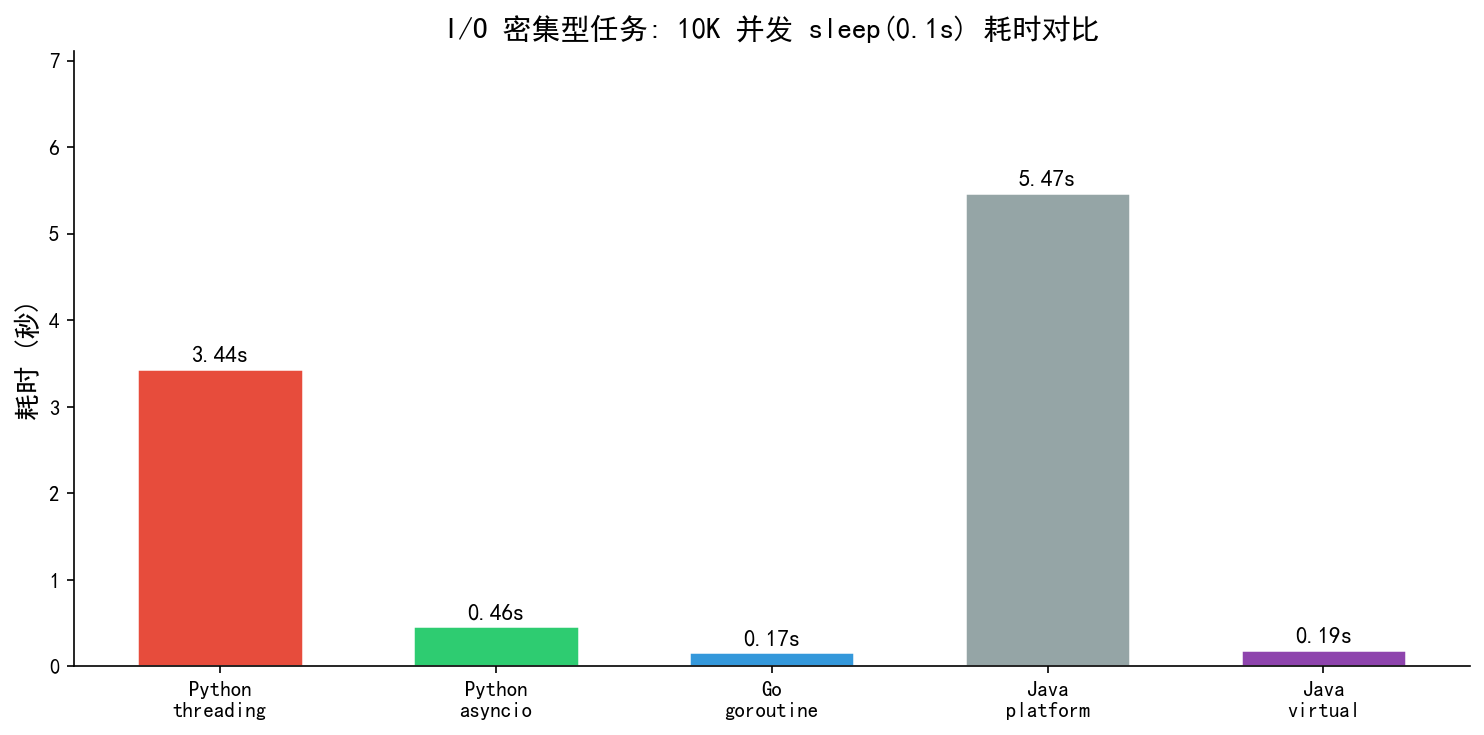
\includegraphics[width=0.92\linewidth]{io_throughput.png}
    \end{column}
    \begin{column}{0.36\linewidth}
      \smallpoint{Python}{threading 3.130s\\asyncio 0.446s\\约 7.0$\times$}
      \smallpoint{Go}{goroutine 0.116s}
      \smallpoint{Java}{platform 5.458s\\virtual 0.235s\\约 23.2$\times$}
    \end{column}
  \end{columns}
  \takeaway{优势来自等待期间释放执行权，而不是把 sleep “算得更快”。}
\end{frame}

\begin{frame}{真实本地 TCP：优势变小，但结论更真实}
  \begin{columns}[T,totalwidth=\linewidth]
    \begin{column}{0.48\linewidth}
      \begin{table}
        \small
        \begin{tabular}{l r}
          \toprule
          模型 & 1000 次 TCP echo \\
          \midrule
          Python asyncio & 1.632$\pm$1.119 s \\
          Python threading & 1.948$\pm$0.303 s \\
          \bottomrule
        \end{tabular}
      \end{table}
      {\small asyncio 约为 threading 的 1.2$\times$。}
    \end{column}
    \begin{column}{0.48\linewidth}
      \begin{block}{为什么这页重要}
        \begin{itemize}
          \item 加入 loopback socket 的 connect/write/read/close；
          \item 优势小于 sleep 微基准；
          \item 真实服务还会有 HTTP/TLS、数据库和序列化开销。
        \end{itemize}
      \end{block}
    \end{column}
  \end{columns}
\end{frame}

\begin{frame}{CPU 密集 + 切换开销：协程不加速计算}
  \begin{columns}[T,totalwidth=\linewidth]
    \begin{column}{0.50\linewidth}
      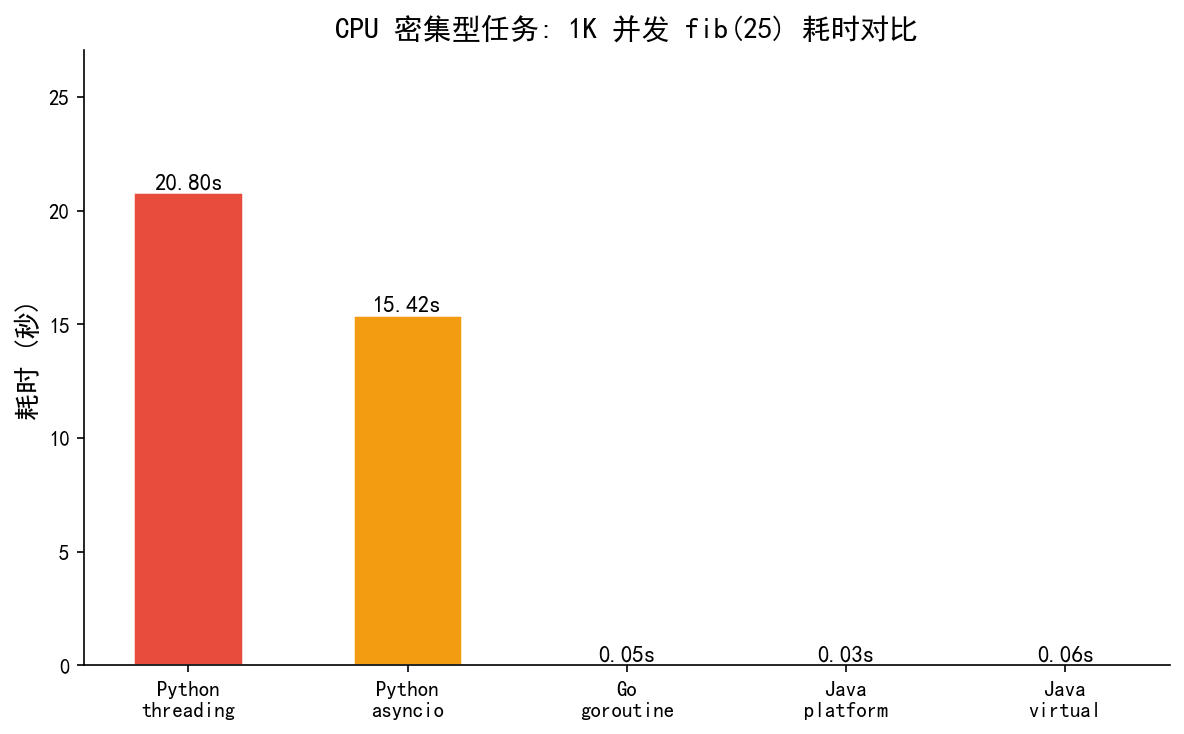
\includegraphics[width=0.93\linewidth]{cpu_benchmark.png}
      \vspace{0.05cm}
      {\scriptsize Go / Java 快主要来自多核并行，不是协程改变算法复杂度。}
    \end{column}
    \begin{column}{0.46\linewidth}
      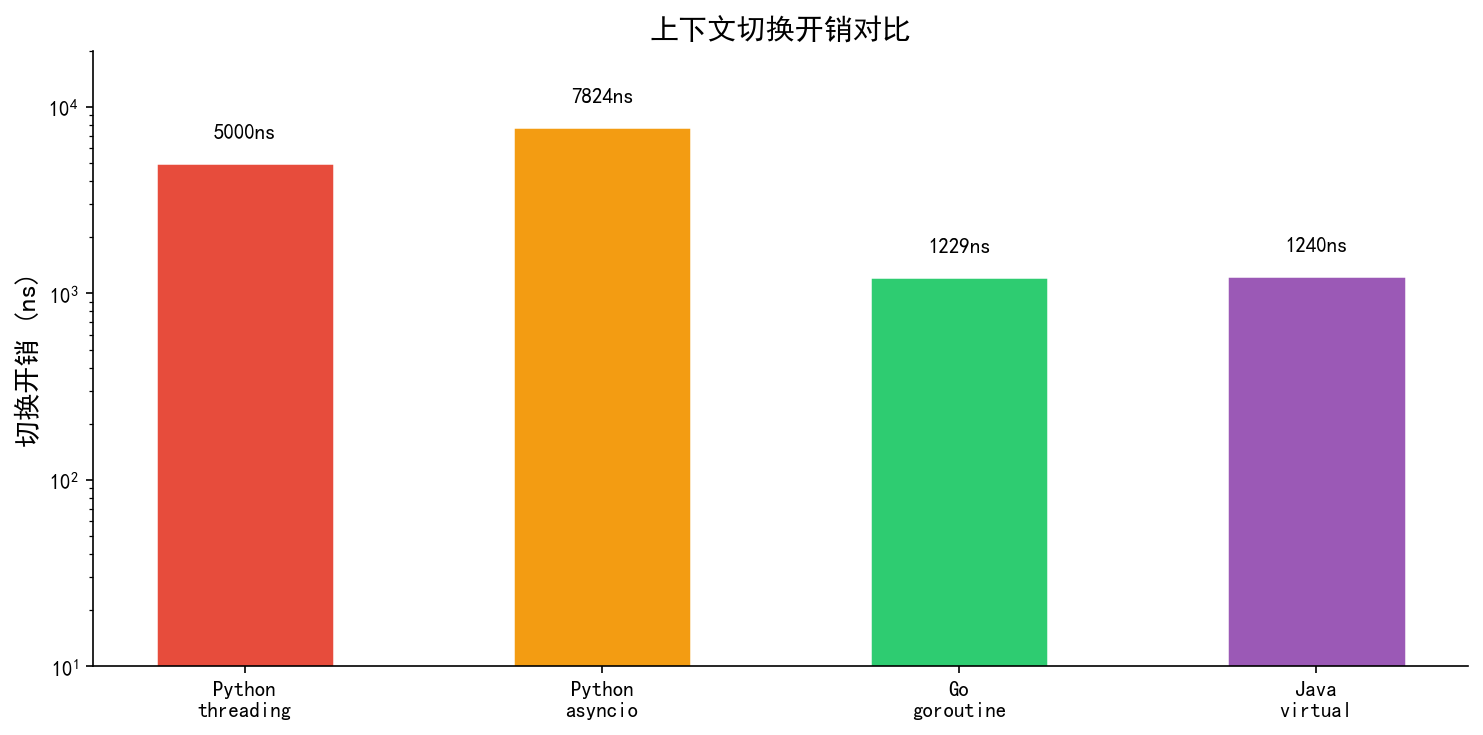
\includegraphics[width=0.93\linewidth]{switch_overhead.png}
      \vspace{0.05cm}
      {\scriptsize 微基准不完全同构，只用于量级讨论。}
    \end{column}
  \end{columns}
  \begin{alertblock}{解释边界}
    协程能减少等待占用的线程资源，但不能减少斐波那契递归本身的指令数。
  \end{alertblock}
\end{frame}

\begin{frame}{Java pinning：虚拟线程也有硬边界}
  \begin{columns}[T,totalwidth=\linewidth]
    \begin{column}{0.46\linewidth}
      \begin{table}
        \small
        \begin{tabular}{l r}
          \toprule
          模式 & 120 个任务 \\
          \midrule
          virtual thread 普通 sleep & 125$\pm$12 ms \\
          synchronized 内 sleep & 3237$\pm$5 ms \\
          \bottomrule
        \end{tabular}
      \end{table}
      {\small 调度器并行度设为 4；pinning 约慢 25.9$\times$。}
    \end{column}
    \begin{column}{0.50\linewidth}
      \begin{alertblock}{解释}
        如果只有 4 个 carrier 能并行承载被固定的阻塞任务，120 个 100ms sleep 至少约需 3000ms；实测 3237ms 与机制一致。
      \end{alertblock}
      \takeaway{virtual thread 降低阻塞等待成本，但不是让所有阻塞都无代价。}
    \end{column}
  \end{columns}
\end{frame}

\begin{frame}{内存使用：只能看趋势，不能简单排名}
  \begin{columns}[T,totalwidth=\linewidth]
    \begin{column}{0.55\linewidth}
      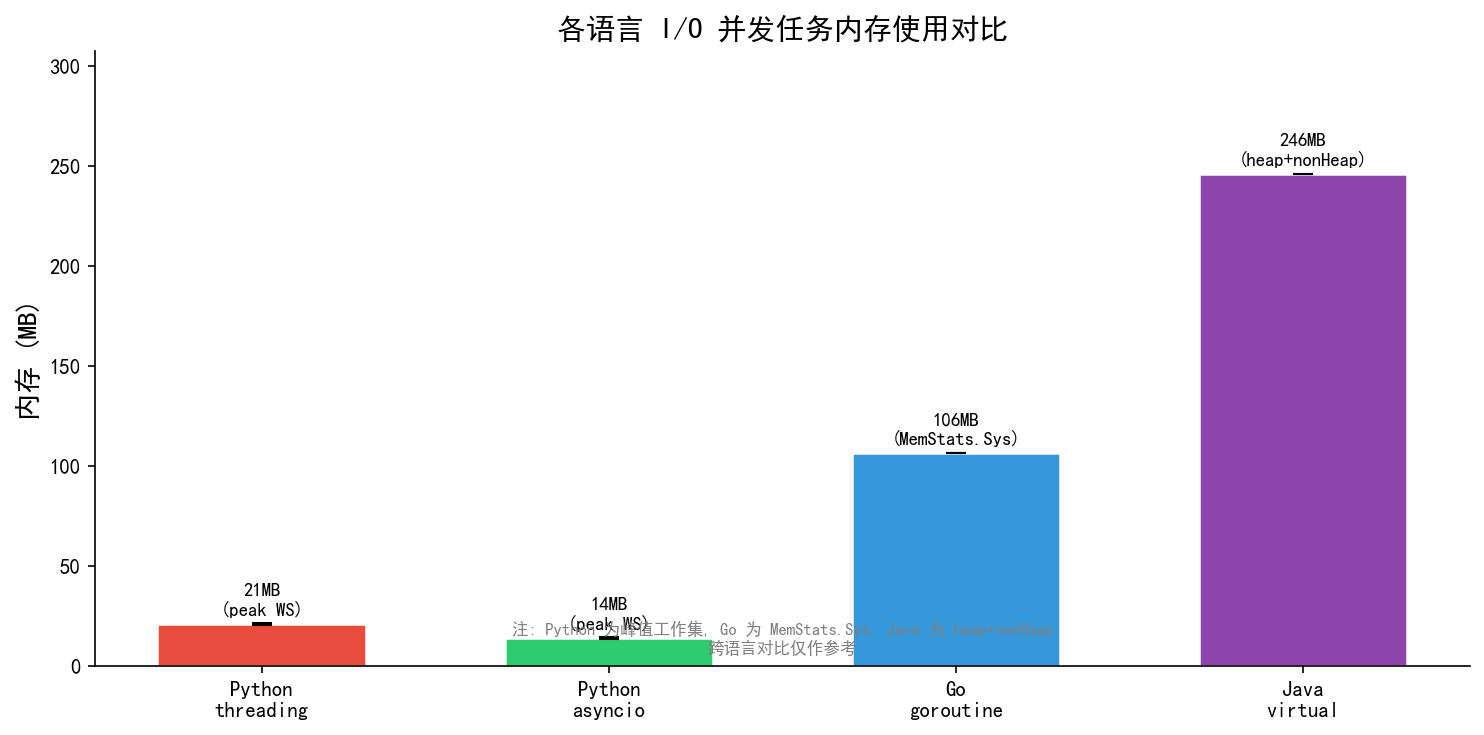
\includegraphics[width=0.96\linewidth]{memory_usage.png}
    \end{column}
    \begin{column}{0.40\linewidth}
      \begin{block}{测量口径}
        \begin{itemize}
          \item Python：进程峰值 working set；
          \item Go：\texttt{runtime.MemStats.Sys}；
          \item Java：heap + nonHeap；
          \item 跨语言对比只看数量级。
        \end{itemize}
      \end{block}
    \end{column}
  \end{columns}
  \takeaway{Python frame 小不等于语言总是最省内存；Go/Java 图中包含运行时、GC、JIT 等系统成本。}
\end{frame}

\begin{frame}{实验有效性：这组数据能说明什么}
  \small
  \begin{itemize}
    \item \textbf{内部有效性}：基础微基准和 TCP echo 重复 5 次，pinning 重复 3 次，给出均值和标准差。
    \item \textbf{构造有效性}：sleep 隔离等待承载能力；TCP 加入 socket 生命周期；pinning 验证 synchronized 阻塞边界。
    \item \textbf{外部有效性}：绝对数值会受 Windows IOCP、JVM 参数、Go/Python 版本和真实网络影响。
    \item \textbf{结论边界}：能证明 I/O 等待中轻量任务更省线程资源；不能证明协程自动加速 CPU。
  \end{itemize}
  \begin{alertblock}{仍未覆盖}
    完整 HTTP server、TLS、数据库连接池、日志、序列化和端到端背压。
  \end{alertblock}
\end{frame}

\section{选型建议与总结}

\begin{frame}{场景化选型：按工作负载选择}
  \scriptsize
  \begin{tabularx}{\linewidth}{l Y Y}
    \toprule
    场景 & 推荐方向 & 主要理由与注意事项 \\
    \midrule
    CPU 密集计算 & 多线程/多进程/SIMD/GPU & 协程不能减少计算量，只能改善等待与调度开销。 \\
    新建高并发后端 & Go goroutine & GMP、netpoller 与标准库协同成熟。 \\
    JVM 旧系统迁移 & Java 21 virtual thread & 同步代码改造成本低，但要关注 synchronized、JNI 和 pinning。 \\
    Python Web/爬虫 & asyncio/FastAPI/uvloop & 上手快，生态成熟；必须避免同步阻塞进入事件循环。 \\
    系统级低延迟服务 & Rust tokio 或 C++20 + asio/io\_uring & 控制力强、开销低，但学习和工程复杂度更高。 \\
    \bottomrule
  \end{tabularx}
\end{frame}

\begin{frame}{三个问题快速判断}
  \begin{enumerate}
    \item \textbf{瓶颈是否真的在 I/O 等待？}\\
    {\small 如果瓶颈在 CPU，优先考虑多线程、多进程、SIMD、GPU 或算法优化。}
    \vspace{0.2cm}
    \item \textbf{阻塞 API 能否被运行时接管或替换？}\\
    {\small Go / Java 21 更适合保留同步写法；C++ / Python / Rust 往往需要显式 async 化。}
    \vspace{0.2cm}
    \item \textbf{错误、取消、超时和背压能否结构化管理？}\\
    {\small 没有这层治理，协程越轻量，系统越容易积累后台任务。}
  \end{enumerate}
  \takeaway{三问都能肯定回答时，协程通常比传统线程池更适合高并发 I/O。}
\end{frame}

\begin{frame}{结论}
  \begin{block}{结论 1：协程承载大规模 I/O 并发}
    它降低的是“等待”的代价，不是“计算”的代价。
  \end{block}
  \begin{block}{结论 2：协程需要三层系统协同}
    编译器/解释器、语言运行时、OS I/O 多路复用共同完成挂起与恢复。
  \end{block}
  \begin{block}{结论 3：选型要看边界}
    sleep 微基准能证明等待承载能力；TCP 和 pinning 实验提醒我们，真实系统还要看协议栈、锁、native 调用和取消语义。
  \end{block}
\end{frame}

\section{AI 使用说明}

\begin{frame}{AI 使用与参考资料}
  \begin{columns}[T,totalwidth=\linewidth]
    \begin{column}{0.49\linewidth}
      \begin{block}{AI 使用说明}
        \begin{itemize}
          \item 辅助梳理“引言-机制-语言-实验-选型”的展示结构；
          \item 辅助检查术语一致性、长句拆分和图表说明；
          \item 实验数据由本机实际运行得到，结论人工复核。
        \end{itemize}
      \end{block}
    \end{column}
    \begin{column}{0.47\linewidth}
      \begin{exampleblock}{主要参考}
        Conway 1963；de Moura \& Ierusalimschy 2009；JEP 444；PEP 492；C++20 coroutines；Python asyncio TaskGroup；Go runtime。
      \end{exampleblock}
      \vspace{0.35cm}
      \centering
      {\Huge\bfseries 谢谢！\par}
    \end{column}
  \end{columns}
\end{frame}

\end{document}
